% Very simple template for lab reports. Most common packages are already included.
\documentclass[a4paper, 11pt]{article}
\usepackage[utf8]{inputenc} % Change according your file encoding
\usepackage{float}
\usepackage{graphicx}
\usepackage{url}
\usepackage{xcolor}
\usepackage{colortbl}
\usepackage{array}
\usepackage{tikz}
\usepackage{subcaption}
\usepackage{enumitem}

% Define the color gradient
\definecolor{darkgreen}{RGB}{26, 188, 156}
\definecolor{medgreen}{RGB}{52, 211, 153}
\definecolor{lightgreen}{RGB}{132, 204, 22}
\definecolor{yellow}{RGB}{250, 204, 21}
\definecolor{orange}{RGB}{251, 146, 60}
\definecolor{red}{RGB}{239, 68, 68}

%opening
\title{HW5 Report, Chordy: A Distributed Hash Table}
\author{David Fischer}
\date{\today{}}

\begin{document}

\maketitle

\section{Introduction}
This assignment's goal was the implementation of \textit{Chordy} a DHT based on a variation of \textit{Chord}, a distributed lookup protocol designed to efficiently identify the node in a peer-to-peer that stores a particular data item.
\textit{Chord} addresses many problems distributed systems face such as load balancing, decentralization, scalability, availability, and flexible naming.

\section{Implementation}

\subsection{Ring Structure}

To ease validation and development, instead of the usually intended consistent hashing function, simple numerical IDs were used for both nodes and later on keys. This still provides the random distribution of keys to nodes, which should result in even storage sizes between nodes.
% As before, let m be the number of bits in the key/node identifiers. Each node, n, maintains a routing table with (at most) m entries, called the finger table.
As opposed to the \textit{finger table}, used in the original \textit{Chord} paper, which allows for $O(log N)$ lookup times, a simpler routing table was implemented. Each node only keeps track of its successor and predecessor in the ring. This results in $O(N)$ lookup times.
The ring structure is periodically stabilized through a \texttt{stabilize/3} function, which gradually heals the ring when new nodes join by having each node ask its successor for their predecessor and adjusting its own records accordingly.
As the structure will have to wrap around at some point, the \texttt{between/3} function was implemented in a way to handle \texttt{From} being larger than \texttt{To} by checking if the \texttt{Id} is either larger than \texttt{From} or smaller than \texttt{To}.

\subsection{Storage}

Storage was implemented by having each node keep a map of key-value pairs which can be added and looked up by sending corresponding messages to the nodes.
These messages are routed through the ring structure until they reach the node responsible for the given key,
at which point the operation is executed and the client is notified through a message including the reference it provided using \texttt{make\_ref/0}.
Additionally, to support new nodes joining the ring, a handover message containing the keys split from the predecessor, based on the two nodes keys, is sent to the new node.

\subsection{Failure Detection}

To detect failed nodes, Erlangs failure detection mechanism was used to have each node monitor their predecessor and successor.
Nodes keep a record of their successors successor, which is provided during each stabilization round. This is done to maintain structure should their original successor fail.
Should the predecessor fail, nodes set it to \texttt{nil} and wait for the predecessors predecessor to notify them.
This approach is however not ideal if two neighboring nodes fail concurrently.

\subsection{Data Replication}

As data is only stored in memory, node failures result in data loss. To mitigate this, nodes keep a replica of their predecessors data which is built concurrently with the main storage.
The client is only notified of a successful add operation once both the main storage and the replica have been updated.
Both the handover and failure handlers were updated to correctly split and merge the replica storage depending on the state of the ring.
In simple terms, when a predecessor dies, the node merges the replica storage with its main storage and propagates its new state to its successor.
When a new node joins, it receives the relevant keys for both its main storage and replica storage from its predecessor.

\section{Main problems and solutions}

\subsection{Functions and Parameters}

The amount of functions and parameters the mature implementations require posed difficulties with retaining a holistic view and often lead to failing tests due to return value mismatches and bugs. 
This was resolved through meticulous analysis and stepping through the node implementations function for function.

\subsection{Replication}

Implementing functional data replication posed the greatest challenge as it required considerations in every part of the system.
A rudimentary early implementation used the synchronization cycles to periodically correct the replicas, however this was inefficient and would strain the network. 
Stepping through the implementation scenario for scenario helped identify the necessary changes and a corresponding sketch was created in parallel to aid development, see Figure \ref{fig:replication-sketch}.

\section{Evaluation}

\subsection{Performance}

% xxx something on scale affecting the performance in both directions.
Figure \ref{fig:heatmaps} shows the performance of the DHT with different ring sizes and amounts of clients, each of the client machines performing 1000 operations over the first node in the ring.
The heatmaps illustrate the routing tables $O(N)$ lookup times, as performance degrades more with the number of nodes in the ring than with the number of clients.
The single entrypoint into the ring is also bottleneck which could be resolved by having clients randomly hit nodes to profit from the pseudo-random key distribution.

\subsection{Ring Maintenance}

When a ring is stabilized on a short delay, the convergence is sped up and thus lookup and add operations get to the correct node faster. Key responsibility and handovers are also sped up.
This however causes the system to use more resources both in terms of compute and network usage, specifically nodes generating messages for \textit{request}, \textit{notify}, and \textit{status} each round.

\section{Conclusions}

The advantages of this distributed storage come both in performance, through load balancing, and fault tolerance, through self healing and the lack of a single point of failure.
Fault tolerance should be however prioritized, especially in productive applications, as data loss is often not acceptable.

Future improvements to the system include routing table improvements with a solution as the \textit{finger table} to improve lookup timings and considering network latency, although this would significantly increase complexity.
A better replica mechanism which is either periodically synchronized through the stabilize function, or persisted on disk which nodes automatically restarting and recovering their state. Replicas could also be used to improve read performance, although this requires dealing with consistency issues.
Finally, either an eventual consistency model could be applied to improve availability, or two-phase commits to ensure consistency, both excluding the other due to the CAP theorem.

\newpage

\appendix

\section{Performance Heatmaps}

\begin{figure}[htbp]
  \begin{subfigure}[b]{0.48\textwidth}
    \resizebox{\textwidth}{!}{%
    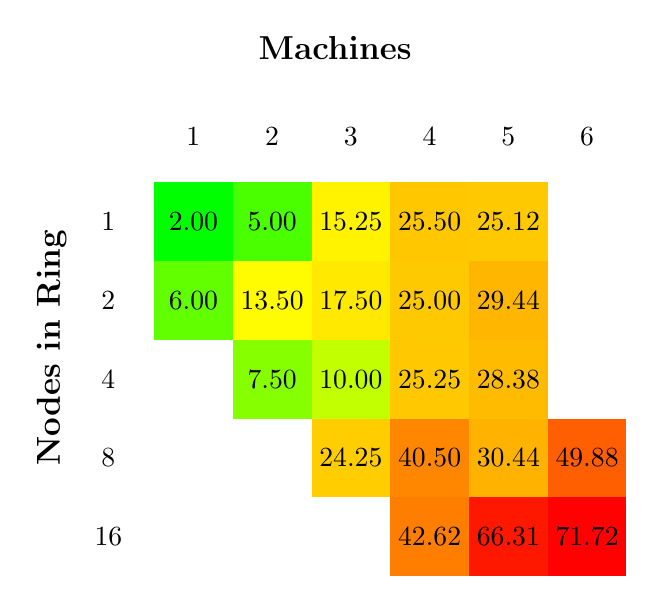
\begin{tikzpicture}[scale=0.8]
      % Label: "Machines" above columns
      \node[font=\large\bfseries] at (3.5, 1.5) {Machines};
      % Label: "Nodes in Ring" to the left of rows
      \node[font=\large\bfseries, rotate=90] at (-1, -3.25) {Nodes in Ring};
      \foreach \y [count=\n] in {
        {2.00,5.00,15.25,25.50,25.12, },
        {6.00,13.50,17.50,25.00,29.44, },
        { ,7.50,10.00,25.25,28.38, },
        { , ,24.25,40.50,30.44,49.88},
        {, , ,42.62,66.31,71.72},
        } {
          % column labels
          \ifnum\n<10
            \node[minimum size=10mm] at (1.25*\n, 0.1) {\n};
          \fi
          % heatmap tiles
          \foreach \x [count=\m] in \y {
            \ifx\x\empty
              % Empty cell - fill with white
              \node[fill=white, minimum size=10mm, inner sep=0pt, outer sep=0pt] 
                    at (1.25*\m,-1.25*\n) {};
            \else
              % Data cell - calculate color
              \pgfmathsetmacro{\normalized}{(\x-2)/(72-2)}
              \pgfmathparse{\normalized<0.15?1:0}
              \ifnum\pgfmathresult=1
                % Low values (0-0.15): green to yellow (very fast transition)
                \pgfmathsetmacro{\r}{\normalized*6.667}
                \pgfmathsetmacro{\g}{1}
                \pgfmathsetmacro{\b}{0}
                \definecolor{cellcolor}{rgb}{\r,\g,\b}
              \else
                % High values (0.15-1): yellow to red
                \pgfmathsetmacro{\r}{1}
                \pgfmathsetmacro{\g}{(1-\normalized)*1.176}
                \pgfmathsetmacro{\b}{0}
                \definecolor{cellcolor}{rgb}{\r,\g,\b}
              \fi
              \node[fill=cellcolor, 
                    minimum size=10mm, text=black, inner sep=0pt, outer sep=0pt] 
                    at (1.25*\m,-1.25*\n) {\x};
            \fi
          }
        }
      % row labels
      \foreach \a [count=\i] in {1, 2, 4, 8, 16} {
        \node[minimum size=10mm] at (-0.1,-1.25*\i) {\a};
      }
    \end{tikzpicture}%
    }
    \caption{Add Operations}
    \label{fig:heatmap-a}
  \end{subfigure}%
  \hfill
  \begin{subfigure}[b]{0.48\textwidth}
    \resizebox{\textwidth}{!}{%
    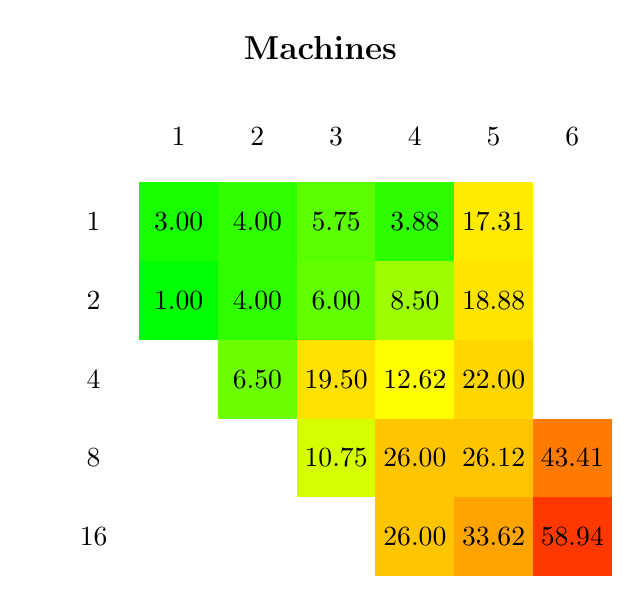
\begin{tikzpicture}[scale=0.8]
      % Label: "Machines" above columns
      \node[font=\large\bfseries] at (3.5, 1.5) {Machines};
      % Label: "Nodes in Ring" to the left of rows
      \node[font=\large\bfseries, rotate=90] at (-1, -3.25) {};
      \foreach \y [count=\n] in {
        {3.00,4.00,5.75,3.88,17.31},
        {1.00,4.00,6.00,8.50,18.88, },
        { ,6.50,19.50,12.62,22.00, },
        { , ,10.75,26.00,26.12,43.41},
        {, , ,26.00,33.62,58.94},
        } {
          % column labels
          \ifnum\n<10
            \node[minimum size=10mm] at (1.25*\n, 0.1) {\n};
          \fi
          % heatmap tiles
          \foreach \x [count=\m] in \y {
            \ifx\x\empty
              % Empty cell - fill with white
              \node[fill=white, minimum size=10mm, inner sep=0pt, outer sep=0pt] 
                    at (1.25*\m,-1.25*\n) {};
            \else
              % Data cell - calculate color
              \pgfmathsetmacro{\normalized}{(\x-2)/(72-2)}
              \pgfmathparse{\normalized<0.15?1:0}
              \ifnum\pgfmathresult=1
                % Low values (0-0.15): green to yellow (very fast transition)
                \pgfmathsetmacro{\r}{\normalized*6.667}
                \pgfmathsetmacro{\g}{1}
                \pgfmathsetmacro{\b}{0}
                \definecolor{cellcolor}{rgb}{\r,\g,\b}
              \else
                % High values (0.15-1): yellow to red
                \pgfmathsetmacro{\r}{1}
                \pgfmathsetmacro{\g}{(1-\normalized)*1.176}
                \pgfmathsetmacro{\b}{0}
                \definecolor{cellcolor}{rgb}{\r,\g,\b}
              \fi
              \node[fill=cellcolor, 
                    minimum size=10mm, text=black, inner sep=0pt, outer sep=0pt] 
                    at (1.25*\m,-1.25*\n) {\x};
            \fi
          }
        }
      % row labels
      \foreach \a [count=\i] in {1, 2, 4, 8, 16} {
        \node[minimum size=10mm] at (-0.1,-1.25*\i) {\a};
      }
    \end{tikzpicture}%
    }
    \caption{Lookup Operations}
    \label{fig:heatmap-b}
  \end{subfigure}
  \caption{Performance comparison in milliseconds with varying numbers of nodes and clients.}
  \label{fig:heatmaps}
\end{figure}

\section{Storage Replication Sketch}
\begin{figure}[H]
  \centering
  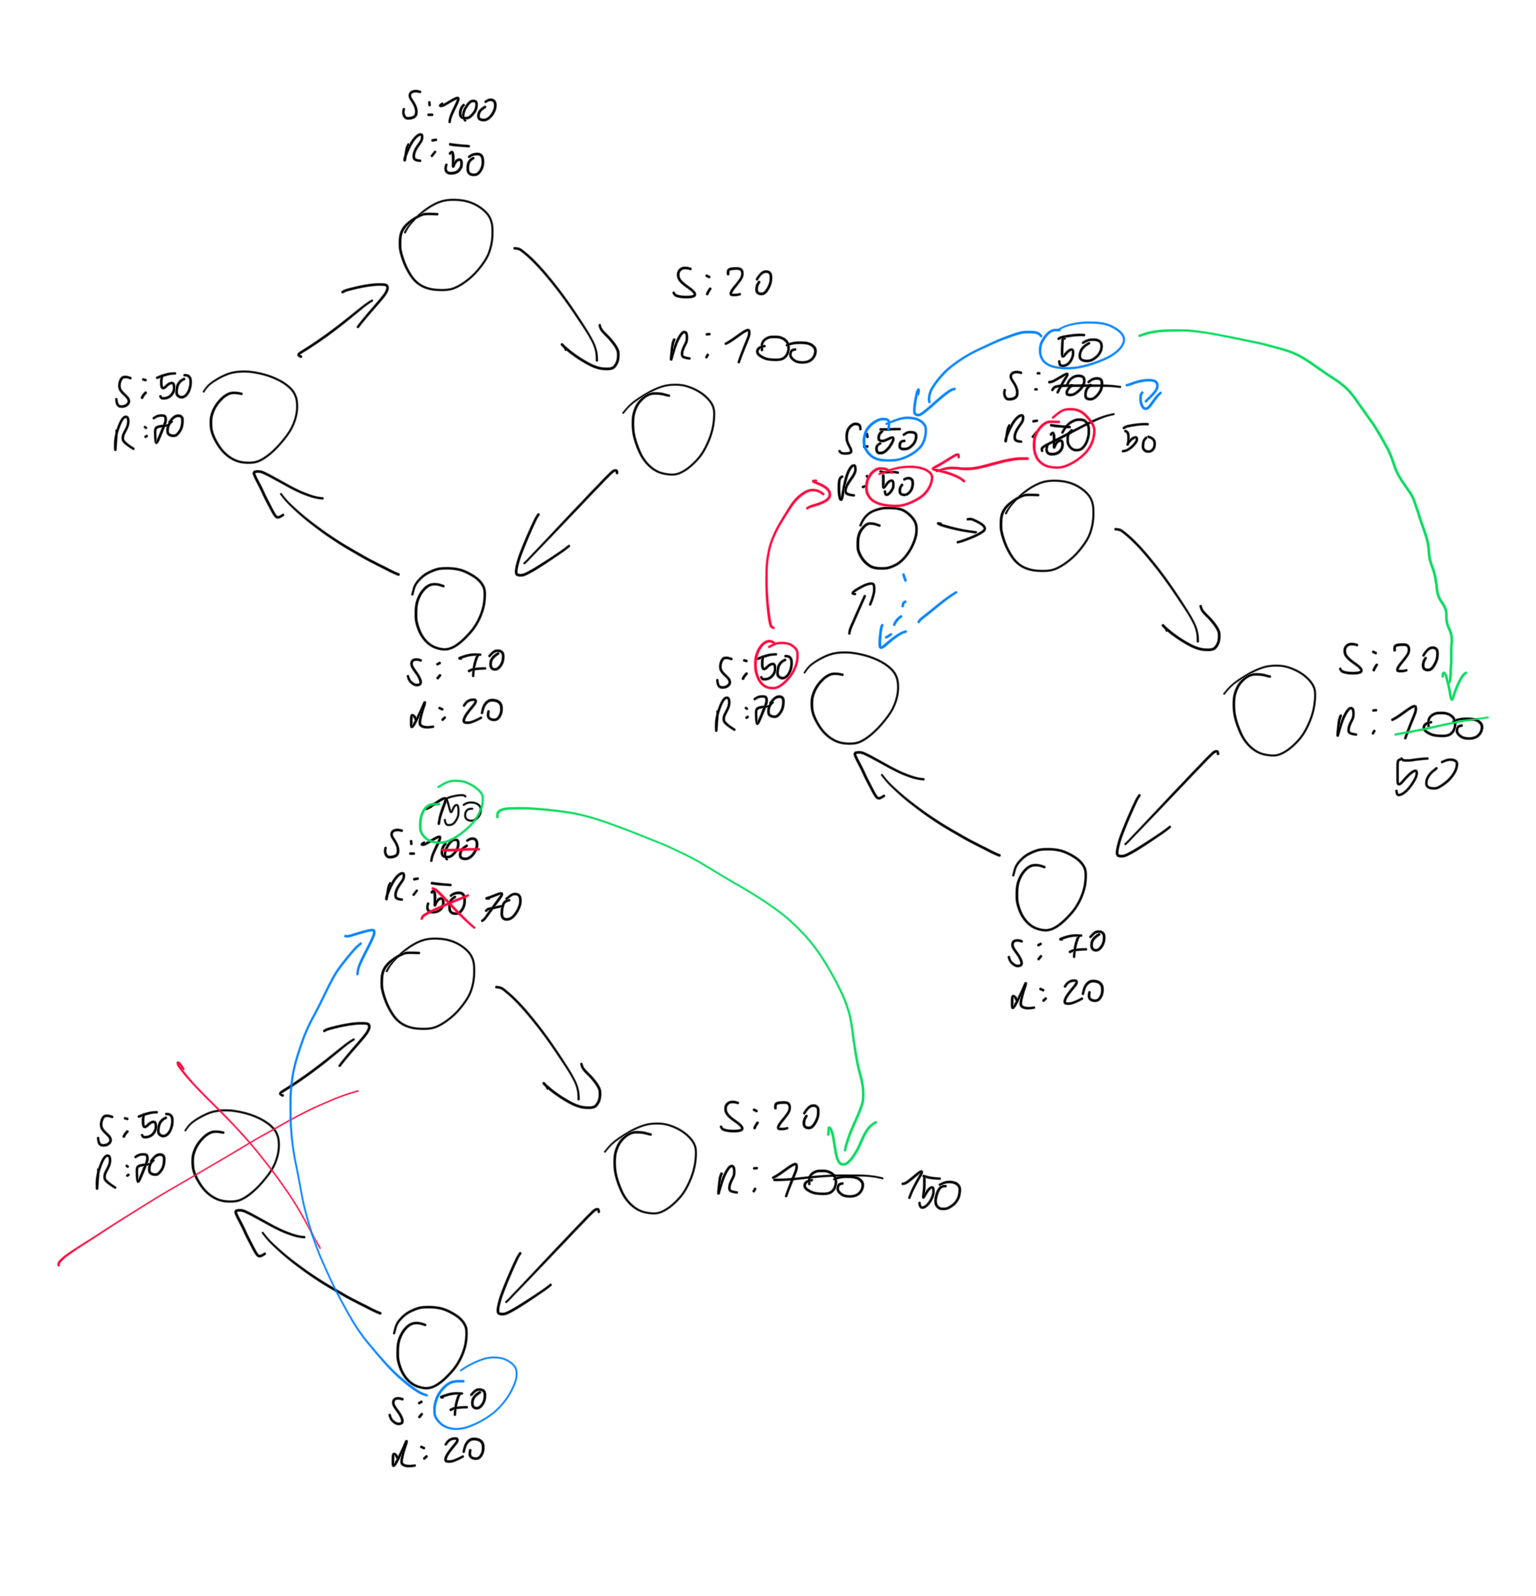
\includegraphics[width=0.7\textwidth]{screenshots/sketch.PNG}
  \caption{Sketch of the replication mechanism.}
  \label{fig:replication-sketch}
\end{figure}

\section{Testing}

\begin{figure}[H]
  \centering
  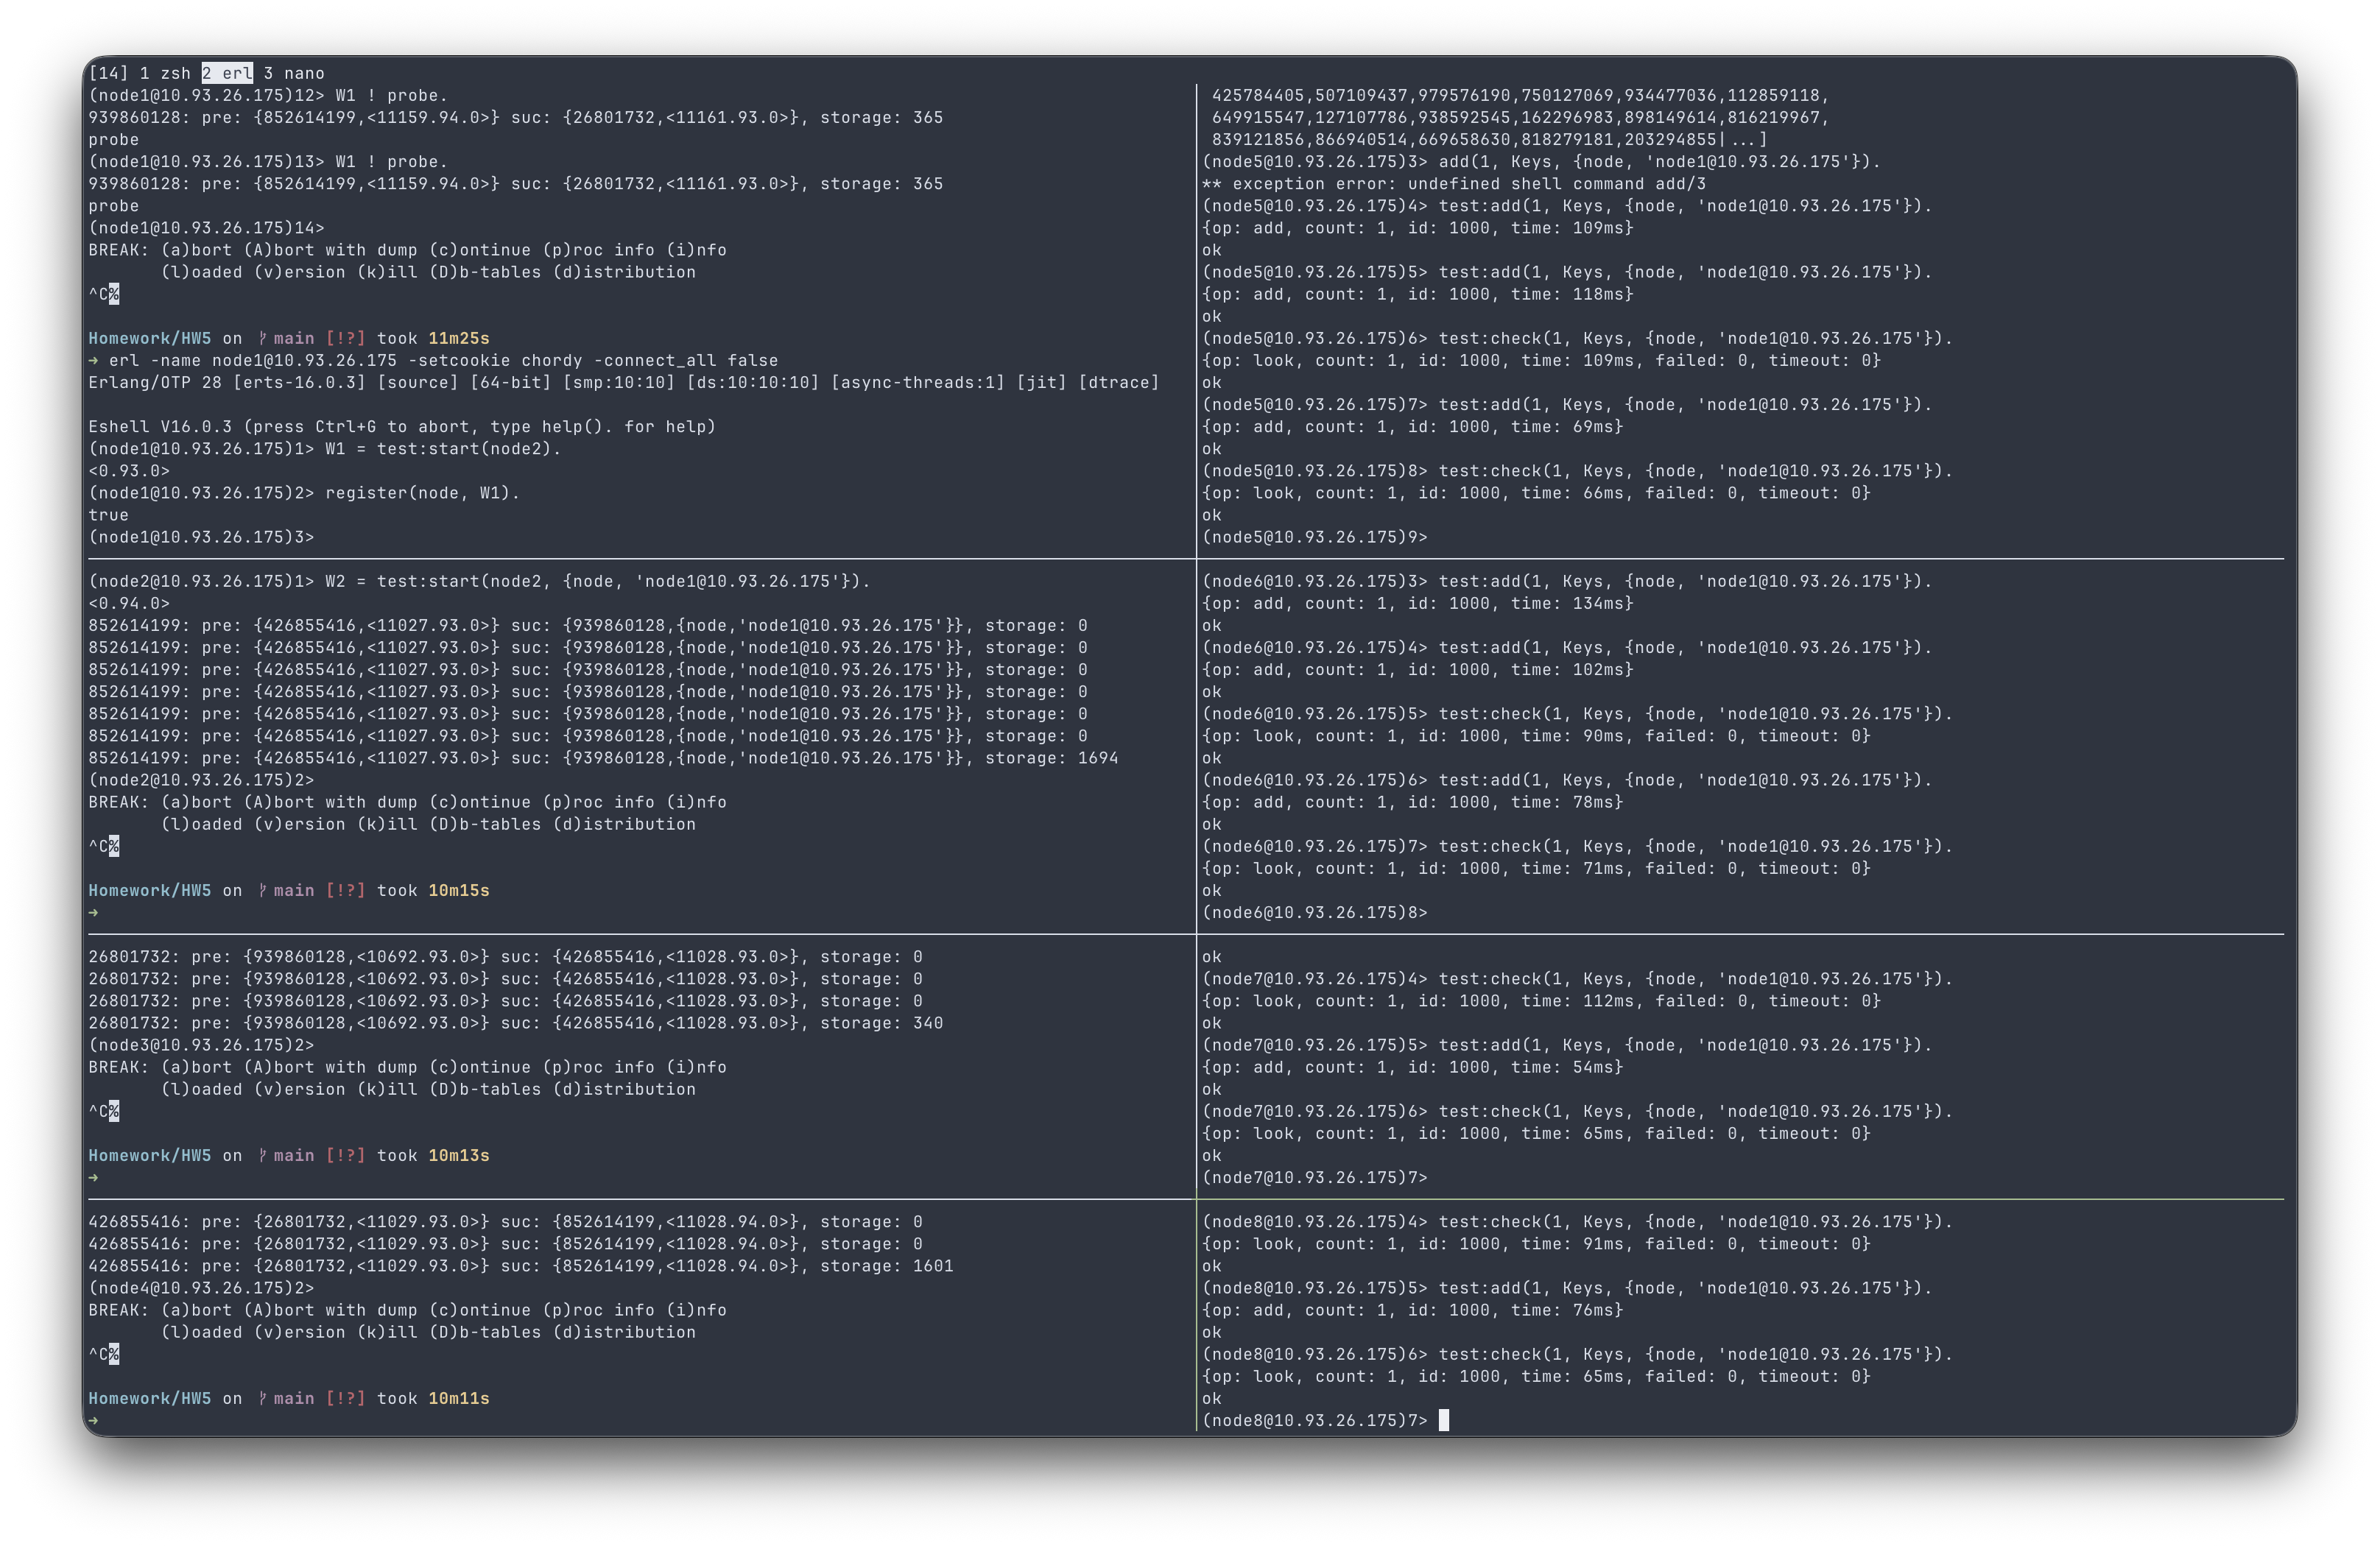
\includegraphics[width=0.9\textwidth]{screenshots/single.png}
  \caption{Single node ring test.}
  \label{fig:test1}
\end{figure}

\begin{figure}[H]
  \centering
  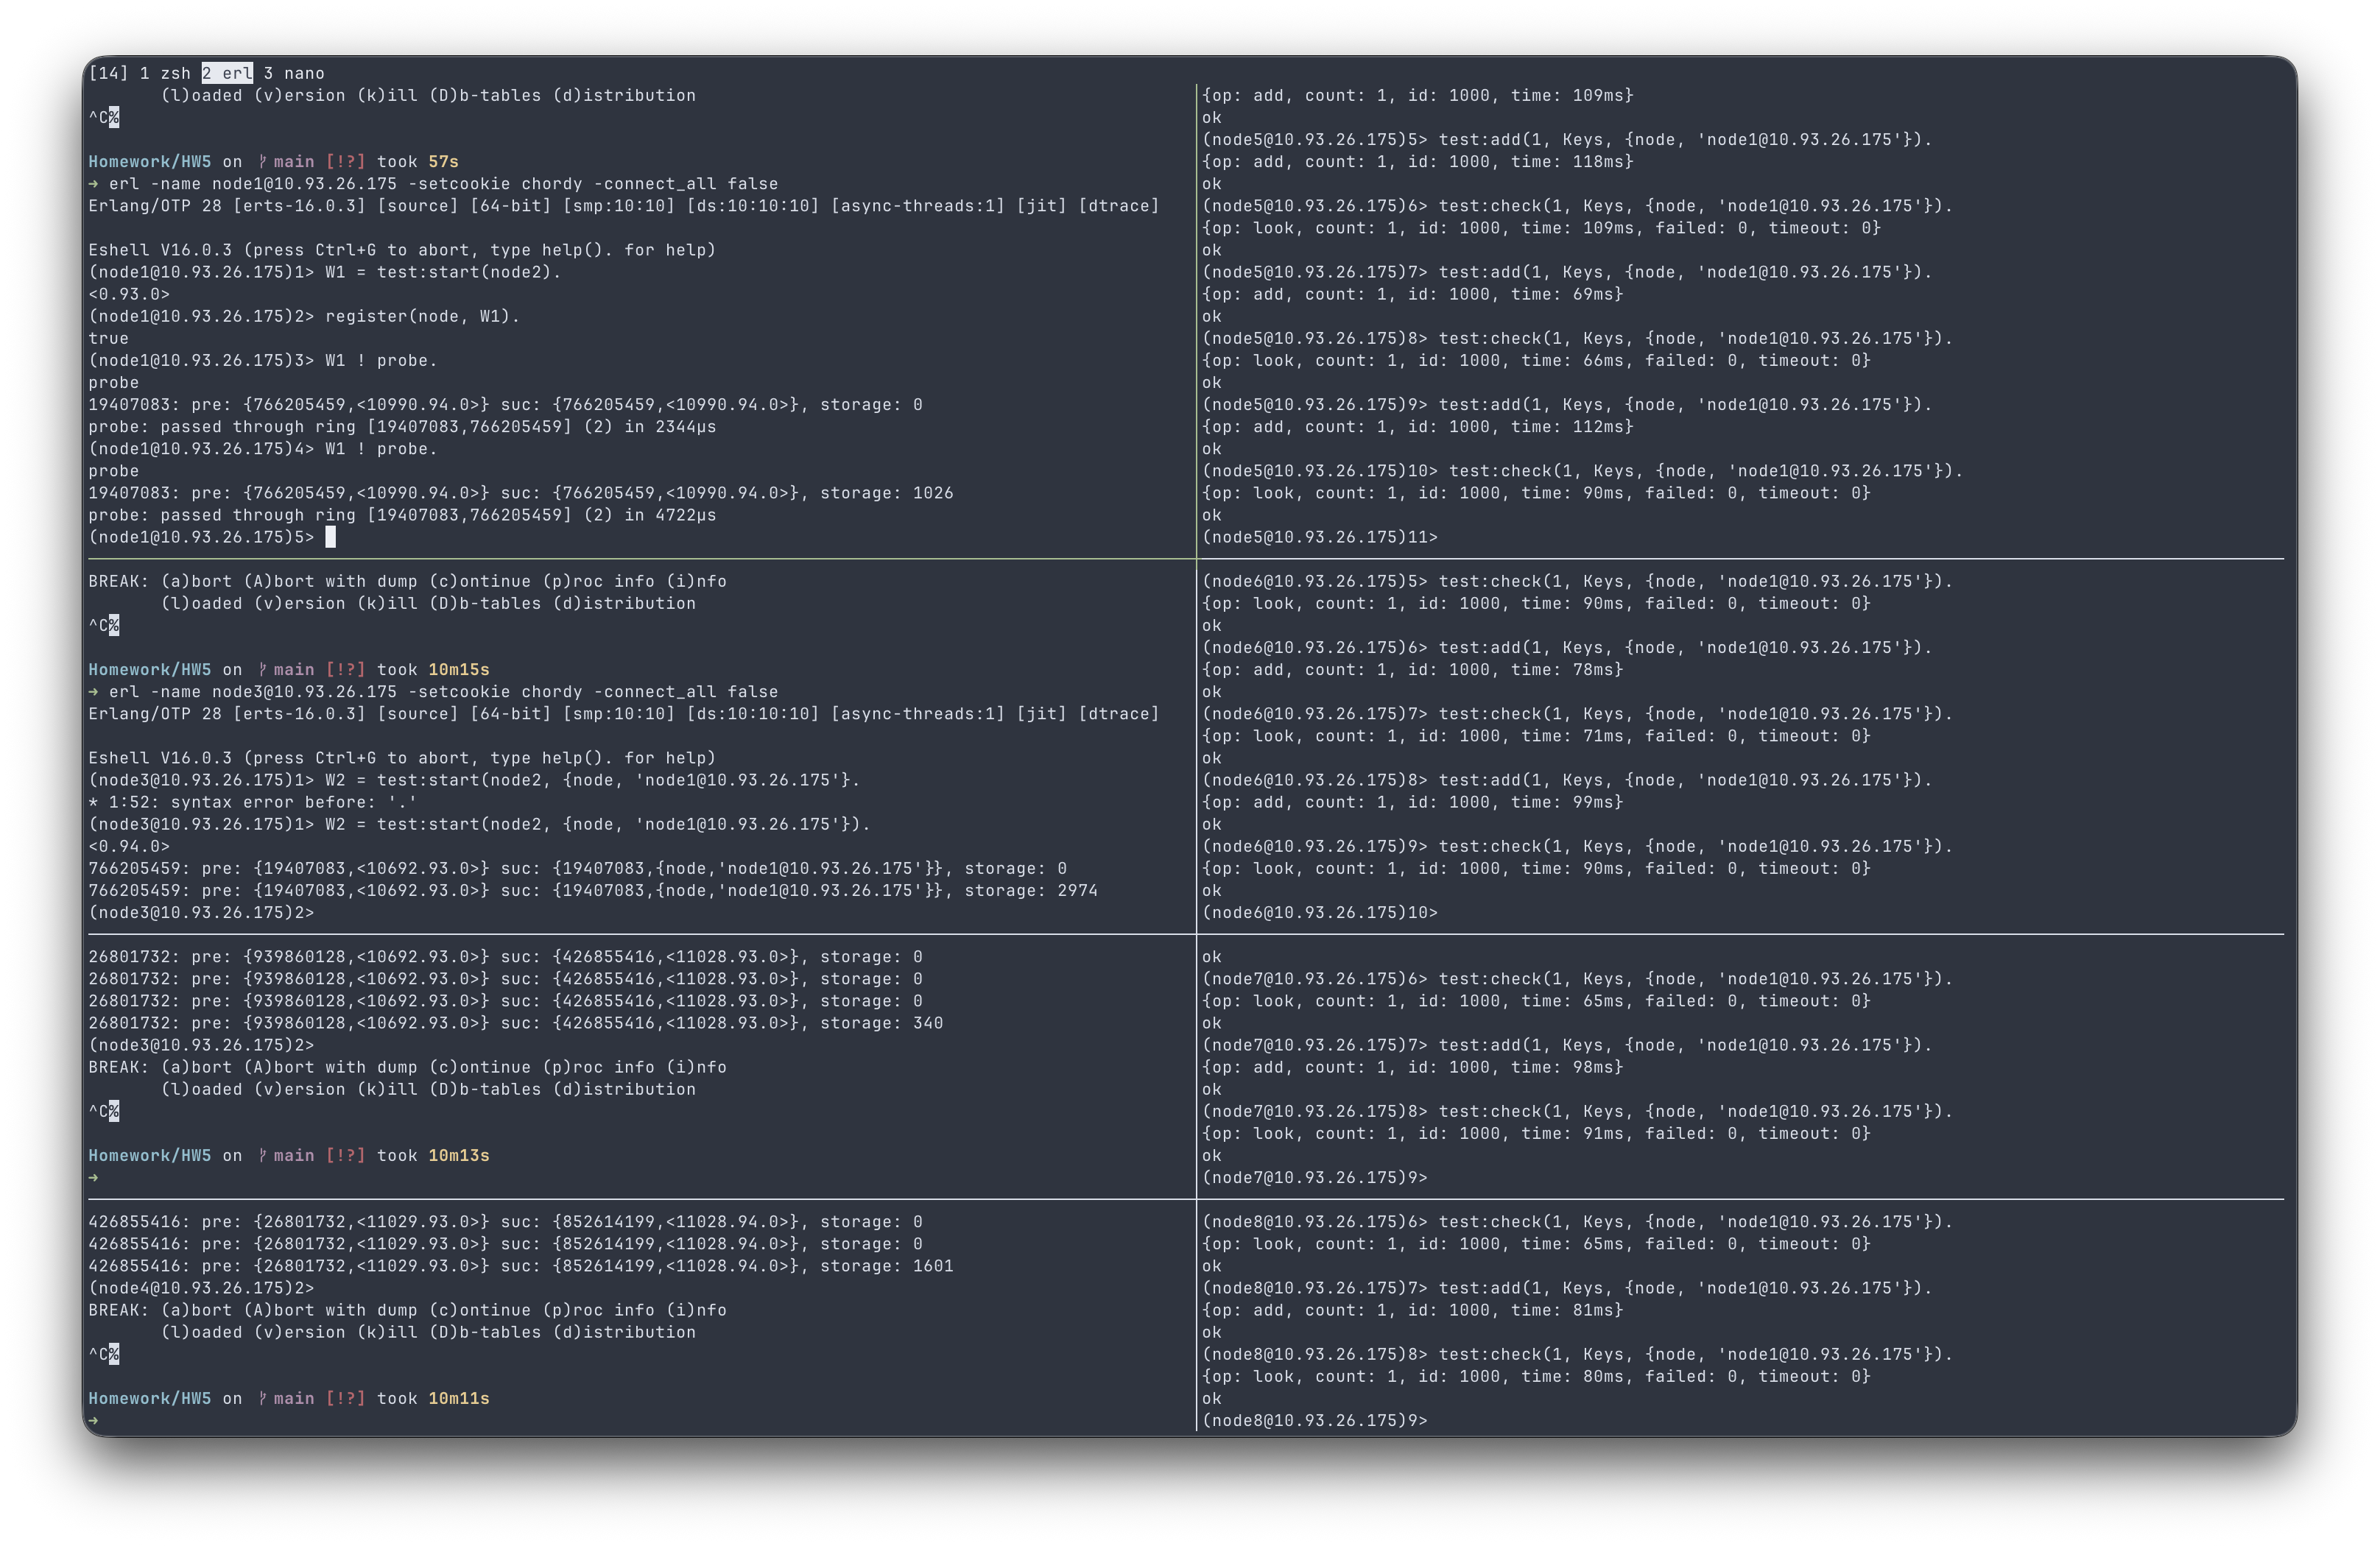
\includegraphics[width=0.9\textwidth]{screenshots/dual.png}
  \caption{Two node ring test.}
  \label{fig:test2}
\end{figure}

\begin{figure}[H]
  \centering
  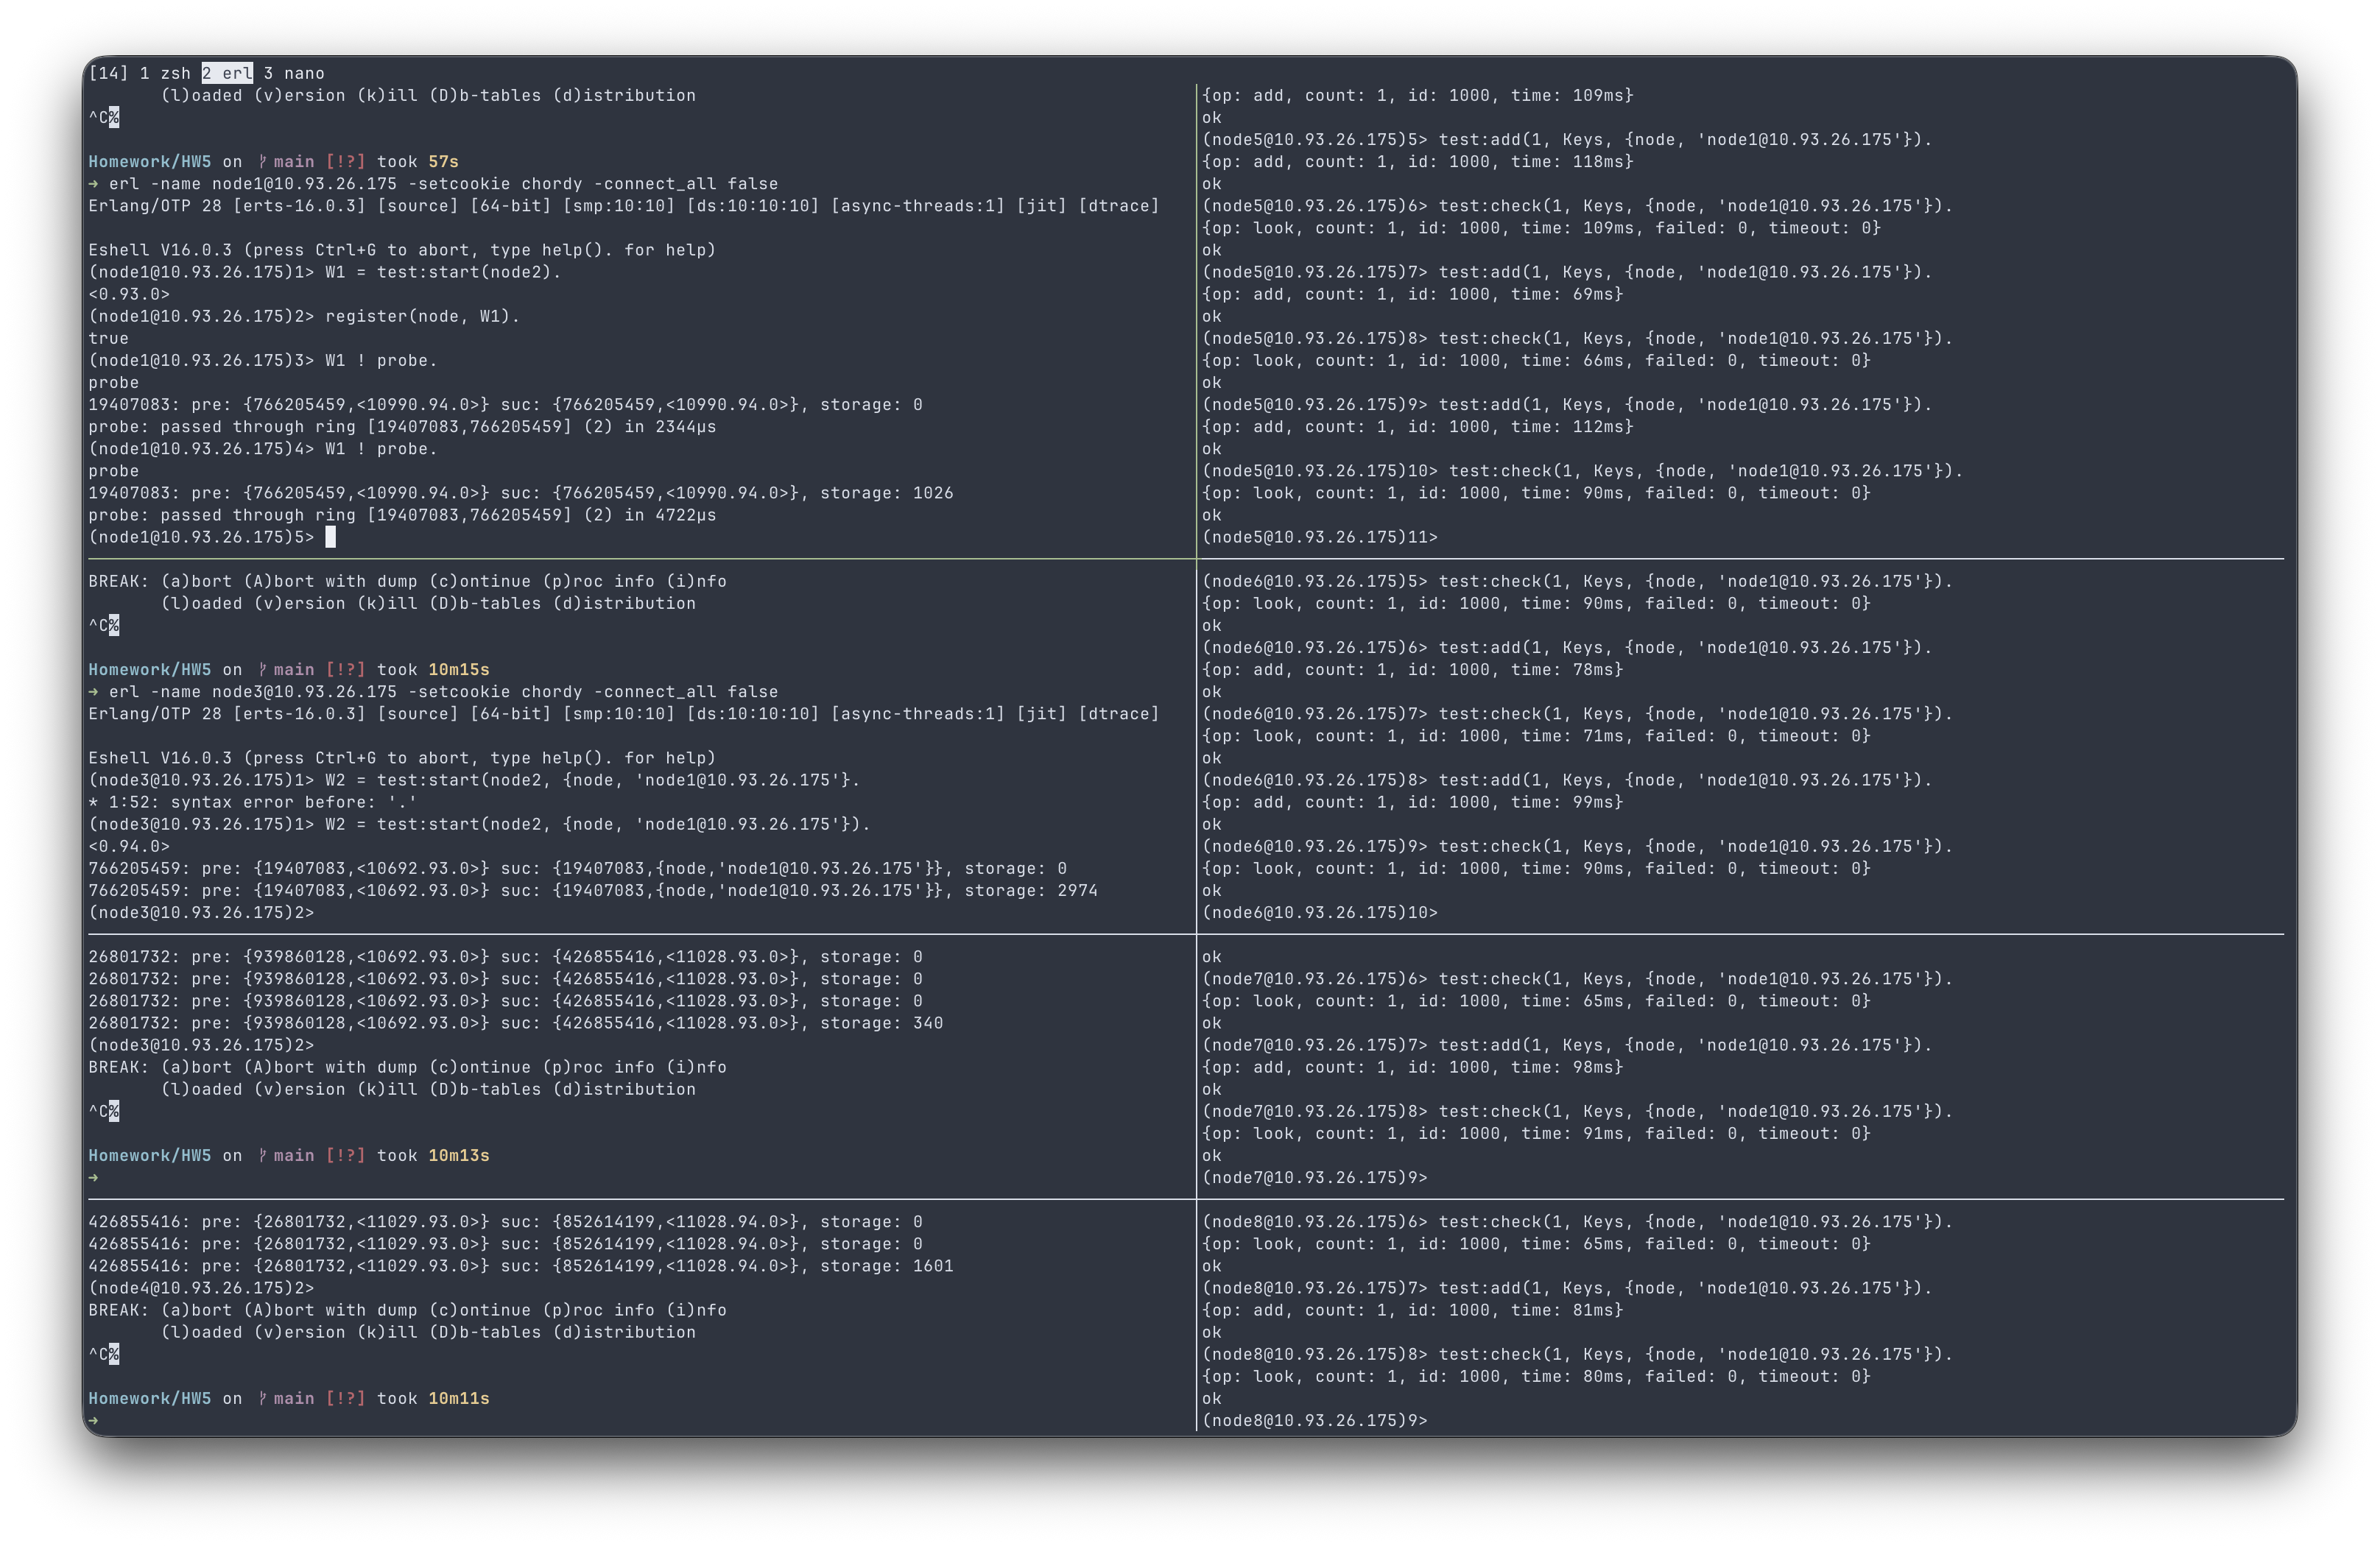
\includegraphics[width=0.9\textwidth]{screenshots/dual.png}
  \caption{Four node ring test.}
  \label{fig:test3}
\end{figure}

\end{document}
